% {\em
% \bit
% \item
% what is the problem
% \item
% what are the applications
% \eit
% }
Today people all around the world use online social networks (OSNs) not only for personal connections but also for entertainment, to share opinions, to read news and inform themselves and to exchange knowledge and information. With their rise in popularity OSNs in the past decade however, they have become a target for abuse by malicious actors who are spamming the network, attempting to scam users, distribute malware, boost a legitimate user's popularity or increase the visibility of certain content. Furthermore with the 2016 United States presidential election the focus has been on social media rather than traditional media for the first time and the concern over widespread \emph{fake news} influencing public opinion as well as social bots pushing state-actor agendas has been growing~\cite{allcott2017social,grinberg2019fake} with some recent research focusing on identifying fake news using data mining methods~\cite{shu2017fake}.

Many OSNs spend a considerable amount of money and time in the form of manual labor on identifying and removing fake accounts. Our goal is to build on previous research and to improve the classification process for more effective and efficient identification of fake accounts. Unlike other approaches which focus on

Given the directed graph $G=(V,E)$ induced by the social network's structure as well as additional classification features $m_v$ for every $v \in V$, we want to identify all nodes $v \in V$ that are likely to correspond to fake accounts. We call this graph a social graph (see \ref{fig:social_graph}. It is however vital that the false-positive rate be kept low as suspensions of legitimate user accounts can degrade the experience enormously.


\begin{figure}
    \centering
    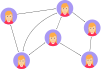
\includegraphics[width=0.4\textwidth]{FIG/social_graph}
    \caption{A social graph}
    \label{fig:social_graph}
\end{figure}

%As public diplomacy or people's diplomacy is broadly being popular, a lot of government-sponsored institutions have bigger chances at communicating directly with foreign publics to establish a dialogue designed to inform and influence with the aim that this foreign public supports or tolerates a government’s strategic objectives. As the international order has changed over the 20th century, so has the practice of public diplomacy. The biggest tool to influence via public diplomacy is social platforms, where we are getting used to bots that are trying to convince us to support some sort of ideas. On this paper we will concentrate on bot detection methods by analyzing the papers and coming to new decisions.
%It has been estimated that around 5-10\text{\%} of all users are bots, and these accounts generate about 20-25\text{\%} of all tweets posted. ~\cite{sysomos} For research purposes, bots present a serious problem because they reduce data accuracy and may dramatically skew the results of analyses using social media. 
%List your main contributions

%The problem we want to solve is the following:
%\bit
%\item GIVEN: a collection of $N$ sound clips, of similar duration,
%      and each having a class label among $k$=5 classes
%\item FIND: a clip-to-clip similarity function
%\item to MINIMIZE: the classification error, in the 1-nearest-neighbor
      classifier.
%\eit

%This is an important problem, because $\ldots$
%millions of dollars $\ldots$
%millions of human lives $\ldots$

The contributions of this project are the following:
\bit
\item our proposed {\em someMETHOD} is novel, combining wavelets
      with a spike-removal  preprocessing step
\item it is effective, achieving 90\% classification accuracy
\item it is scalable, being linear on the number of sound-clips $N$.
\eit

The rest of this paper is structured in the following way: first we do a short survey of related work and their approaches (Section \ref{sec:survey}), based on the findings in these papers we will explore a dataset of Twitter users and fake accounts and their social graph and propose our own method of classifying these accounts, we will test and evaluate our approach in experiments and compare it to other classification approaches.